\chapter{L’aide multicritère à la décision }

\section{Introduction}

Les outils d'aide à la décision permettent d'apporter des réponses pertinentes à des problématiques diverses mettant en œuvre plusieurs choix possibles (implantation de sites industriels, stratégie de dépollution d'un lac, constitution de portefeuilles de valeurs, etc.), d'aider au diagnostic et, plus généralement, de faciliter la prise de décision stratégique ou opérationnelle en environnement imprécis et/ou incertain.\\
La détermination de la « meilleure » action (optimale, de meilleur compromis...) constitue un défi intellectuel perpétuel en sciences et en génie. L’aide multicritère à la décision s’est alors développée pour offrir à la fois une démarche et des outils de solutions à des problèmes décisionnels complexes d’après KEENEY R L. Ainsi, l’analyse multicritère est aujourd’hui considérée comme l’une des branches les plus importantes de la recherche opérationnelle et des théories de la décision.\\
Dans notre cas l’outil d’aide à la décision développé devra aider à la sélection des employés les plus méritants à acquérir une promotion ou prime …  et cela grâce à des méthodes mathématiques d'analyse multicritère qui fournissent un classement des employés.

\section{Définition de l’aide à la décision}
De manière générale l’aide à la décision est l’activité de celui qui, prenant appui sur des modèles clairement explicités mais non nécessairement complètement formalisés, aide à obtenir des éléments de réponses aux questions que se pose un intervenant dans un processus de décision, éléments concourant à éclairer la décision.\\
Elle est généralement sollicitée par des organisations dans le cas où elles sont confrontées à des problèmes complexes, par exemple, de planification, d’allocation et de gestion de ressources, de choix et d’évaluation, etc. Ces problèmes induisent une décision (ou une série de décisions) lourde(s) de conséquences, et que l’expérience et le bon sens, seuls, ne suffisent pas à éclairer. Cette série de décisions s’inscrit dans un processus appelé « processus de décision ».\\
Dans la littérature, il est défini par A. Tsoukiàs comme étant « un espace d’interaction, pouvant évoluer dans l’espace et dans le temps, dans lequel tous les intervenants partagent des préoccupations qui sont parfois contradictoires (améliorer l’approvisionnement, diminuer les coûts) ». L’existence d’un tel espace est justifiée par la présence d’un objectif (préoccupation) final.\\ 
Le fait que le processus de décision soit évolutif, nous laisse supposer que la préoccupation finale peut l’être également. L’aide à la décision, sollicitée par les intervenants dans ce processus, doit aider à répondre, souvent indirectement, à cette préoccupation finale.\\ 
\newpage
L’aide à la décision n’aide pas, nécessairement, à répondre directement à la préoccupation finale mais peut se limiter à certaines questions traduisant les préoccupations de certains intervenants.\\ 
Cependant, nous pensons qu’il est important de s’assurer, en répondant à ces préoccupations, que nous apportons aussi des éléments de réponses à la préoccupation finale et que l’aide à la décision soit cohérente avec l’évolution de cette préoccupation

\section{La problématique de la décision}
La problématique de décision peut être perçue comme étant une orientation de l’investigation qu’on adopte pour un problème de décision donné. Elle exprime les termes dans lesquels le décideur pose le problème et traduit le type de la prescription qu’il souhaite obtenir. Nous pouvons distinguer quatre problématiques en aide multicritère à la décision:
\begin{itemize}
\item Problématique de choix (P.$\alpha$)
\\Elle consiste à sélectionner un sous ensemble aussi restreint que possible de l’ensemble des actions A "une action représente l’objet de la décision", contenant les meilleures actions. L’idéal est d’obtenir une seule et meilleure action. Mais à cause de la nature conflictuelle des critères, il est préférable de fournir au décideur quelques actions qui représentent différentes variantes de la "meilleure action". Évidemment, le résultat final peut être raffiné en utilisant de l’information additionnelle ou avec une analyse plus approfondie. 
\begin{figure}[!h]
\begin{center}
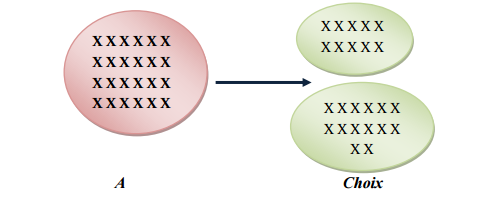
\includegraphics{aide_multicrit_decision/prob_de_choix.png}
\end{center}
\caption{Problématique de choix}
\end{figure}
\item Problématique de tri (P.$\beta$): 
\\Elle consiste à affecter chaque action à un ensemble de catégories prédéfinies. Cette formulation est adéquate lorsque le problème de décision consiste à examiner chaque action indépendamment des autres (en tenant compte que des caractéristiques intrinsèques de chaque action) dans le but de proposer une recommandation parmi un ensemble des recommandations spécifiées en avance. Chaque recommandation peut être associée avec une catégorie. Le problème de décision est alors vu comme trier les actions potentielles aux différentes catégories définies en termes de normes prédéfinies. La procédure de tri doit être définie de telle sorte que chaque action est affectée à une et seule catégorie. Formellement, une prescription consiste à une partition de A.
\begin{figure}[!h]
\begin{center}
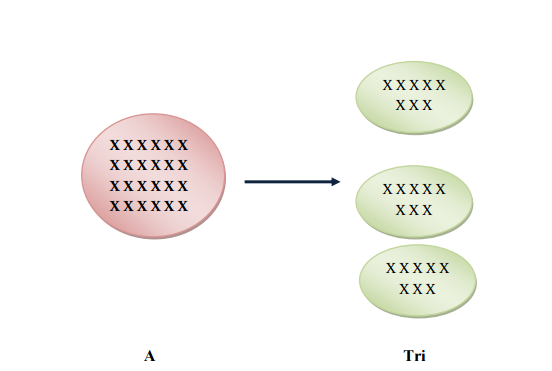
\includegraphics{aide_multicrit_decision/prob_de_tri.png}
\end{center}
\caption{Problématique de tri}
\end{figure}
\newpage
\item Problématique de rangement (P.$\gamma$): 
\\Elle consiste à ranger les différentes actions en allant de la meilleure action à la moins bonne. Cette problématique est intéressante lorsque les actions sont à différencier selon leur intérêt relatif. L’idéal est d’obtenir un ordre complet. Cependant, à cause de la nature conflictuelle des critères, à l’imprécision, à l’existence de systèmes de valeurs différents, il est souvent plus réaliste de présenter au décideur un ordre partiel. Il est à noter qu’en pratique, le rangement peut être nécessaire seulement pour les actions les plus intéressantes. Formellement, la prescription est un ordre partiel, une relation transitive définie sur A (ou un sous ensemble de A).
\begin{figure}[!h]
\begin{center}
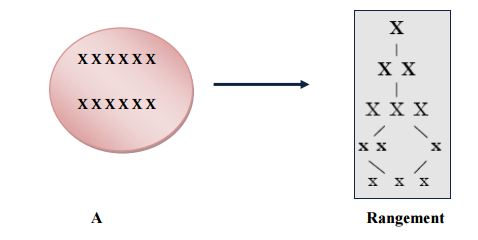
\includegraphics{aide_multicrit_decision/prob_de_rangement.png}
\end{center}
\caption{Problématique de rangement}
\end{figure}
\newpage
\item Problématique de description (P.$\delta$): 
 \\Elle consiste simplement à décrire les actions et leurs conséquences et non pas à les comparer comme c’est le cas avec les trois autres problématiques précédentes. Ici, il n’existe pas une prescription et la procédure d’investigation est cognitive.


\begin{figure}[!h]
\begin{center}
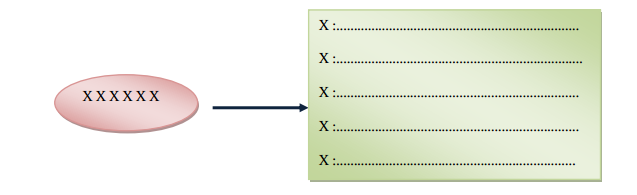
\includegraphics{aide_multicrit_decision/prob_de_descr.png}
\end{center}
\caption{Problématique de description}
\end{figure}
\end{itemize}

Le tableau récapitulatif des quatre problématiques en aide multicritère à la décision d’après B ROY.

\begin{figure}[!h]
\begin{center}
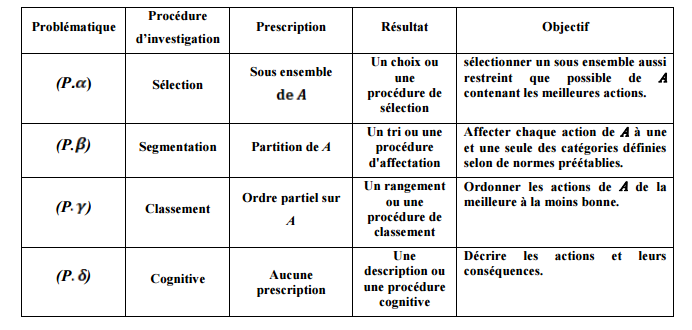
\includegraphics{aide_multicrit_decision/tabl_recap.png}
\end{center}
\caption{Tableau récapitulatif des quatre problématiques}
\end{figure}

Dans notre cas la problématique de mon travail c’est une problématique de rangement, car le but étant de faire un classement des salariés d’une entreprise d’après certains critères.

\newpage
\section{Le processus de décision}
Le processus de décision c’est l’enchaînement des trois phases suivantes d’après SIMON HA: 
\begin{itemize}
\item Phase de compréhension: analyse de la situation et du problème  
\item Phase de modélisation: formulation du problème (mise en évidence des écarts entre la situation actuelle et la situation objectée) et description des solutions potentielles 
\item Phase de sélection: choix d’une solution en fonction de critères concrets (objectifs, normes,…) ou abstraits (intuition, motivation,...), appréhendés par le décideur avec ou sans le soutien d’outils et de techniques d’aide à la décision
\end{itemize}
	
\begin{figure}[!h]
\begin{center}
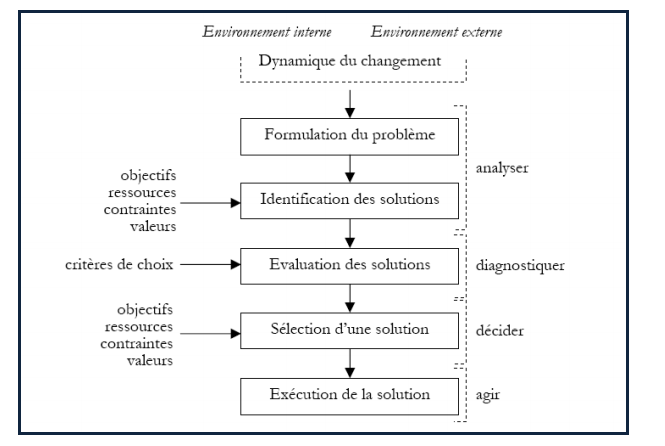
\includegraphics[height=6cm]{aide_multicrit_decision/environement.png}
\end{center}
\caption{Processus de décision}
\end{figure}

\section{Démarche de modélisation}
Dans cette section, nous allons nous intéresser aux types de modèles existants en aide à la décision et plus généralement aux approches fondées sur ces modèles. Il existe plusieurs types de modèles avec leur approche en aide à la décision :
\begin{itemize}
\item Approche normative\\
 Le décideur est rarement sollicité pour la construction de tels modèles. La validité des résultats fournis par le modèle repose sur leur cohérence avec les axiomes de la rationalité économique. Par exemple, on cherche un modèle permettant d’ordonner (du meilleur au moins bon) des investissements selon leur rentabilité économique. Si un investissement a est plus rentable qu’un investissement b et l’investissement b plus rentable qu’un investissement c, alors l’investissement a doit être plus rentable que l’investissement c.
\item Approche descriptive \\
Dans cette approche le décideur n’est également pas directement sollicité pour la mise en œuvre de ces modèles. Ces derniers sont généralement fondés sur des données ou des comportements existants (observations). Ils servent à décrire des phénomènes déjà réalisés pouvant se reproduire dans les mêmes conditions. La validité des résultats fournis par ces modèles repose sur l’observation d’autres phénomènes de même nature.
\item Approche prescriptive \\
L’approche prescriptive se différencie des deux premières par le fait qu’elle ne repose sur aucune information existante (rationalité économique ou observations). L’analyste doit collecter et structurer ces informations afin de construire un modèle. L’intervention du décideur n’est donc pas nécessaire lors de la construction du modèle, néanmoins, il intervient pour sa validation. Par exemple un médecin qui questionne un malade (pouvant décrire correctement ses symptômes mais ne sait pas ce qu’il a) afin de lui prescrire un traitement.
\item Approche constructive \\
La particularité de cette approche est que le décideur est sollicité, à la fois, lors de la construction du modèle mais aussi lors de sa validation. Les modèles sont donc fondés sur les connaissances des décideurs. L’homme d’étude cherche à les expliciter ou à les formaliser. La validation de ces modèles s’effectue, à l’image de l’approche prescriptive, par le décideur. Par exemple, lorsque l’homme d’étude cherche à construire un modèle représentant les préférences d’un décideur.

\end{itemize}

Parmi toutes ces approches, la dernière approche « Approche constructive » est la plus adéquate au travail que je veux effectuer, cela sera explicité en détail dans le chapitre suivant.

\section{Les méthodes multicritères d’aide à la décision}
Le recours aux méthodes multicritères d’aide à la décision s’est largement répandu depuis quelques années. Ces méthodes ont pour but la résolution des problèmes d'Aide à la décision multicritère. \\Elles constituent une étape importante du processus de décision, qui suit celle d'identification et de définition du problème, et aboutissent au choix d'une ou plusieurs solutions optimale(s).\\
Elles permettent également de répondre aux problématiques de tri et de rangement, par l'intermédiaire d'une procédure d'affectation et de classement respectivement.\\
Il existe trois grandes familles de méthodes multicritères. \\La première représente les méthodes utilisant un critère unique de synthèse « Agrégation a priori de critères en un critère unique » dont le principe consiste à agréger les performances d’une alternative en un seul critère. \\La deuxième famille représente les méthodes de sur-classement «Approche fondée sur le sur-classement» dont le principe consiste à comparer les alternatives par paires et enfin les méthodes interactives.\\ 
Nous allons présenter dans cette section les deux premières familles de méthodes, mais tout d’abord introduire quelques définitions importantes a la compréhension de ce qui suit.
\\
Actions, poids et critères de la décision\\
L’action représente l’objet de la décision et afin de différencier les actions réalisables de celles qui ne le sont pas, B. Roy nomme action potentielle ou alternative une action réalisable, c.-à-d. une action dont la mise en œuvre en pratique est envisageable. En aide multicritère à la décision l’ensemble des alternatives A est généralement construit sous forme d’une liste : A = {a1, a2, ...}.\\
Tandis que, un critère g est un outil permettant d’évaluer et de comparer des alternatives « actions » sur un point de vue bien défini. On note g(a) la performance de a sur le critère g, elle représente en général un nombre réel qui prend ses valeurs dans Xg (l’ensemble des valeurs possibles de g) défini explicitement.\\
Le poids quant à lui « w » c’est la valeur qui permet de mesurer l'importance d'un critère par rapport aux autres du point de vue du décideur.\\

\subsection{Agrégation a priori de critères en un critère unique}
Les préférences du décideur sont ramenées à un critère. Facile du point de vue mathématique mais les critères sont amalgamés dans la fonction de réponse. Une solution est présentée comme la meilleure, les actions sont complètement rangées\\
Cette approche englobe plusieurs méthodes « Somme pondérée, Analyse multicritère hiérarchique (AMCH) … »\\
Dans le cadre de mon travail j’ai choisis la somme pondérée et cela pour ça simplicité en terme de modélisation, son efficacité et son accessibilité mathématique.\\


\subsubsection{Somme pondérée}


\setcounter{secnumdepth}{4}


\paragraph{Présentation}
La méthode somme pondérée vise à construire un critère unique g agrégeant les P critères g1, g2, … gP et l’évaluation d’une action a $\epsilon$ A.

\paragraph{Données de départ}
La méthode somme pondérée a besoin de fixer les données de départ suivants :  
\begin{itemize}
\item m actions A1, A2, A3...Am
\item n critères C1, C2, C3...Cn
\item n poids correspondant chacun a un critère, un vecteur poids (W1, W2,...Wn) avec Wj > 0
\item aij = Uj(Ai), fonction d'utilité cardinale quotient, c'est-à-dire que cette fonction représente les écarts en plus de respecter l'ordre et pour laquelle il existe un zéro véritable. Ces données représentent les performances de chaque action sur chacun des critères.
\end{itemize}

\paragraph{Transformation des données}
\begin{enumerate}
\item Normalisation de tous les aij afin de conserver la proportionnalité entre les valeurs.
\item Normalisation des poids (la somme des poids = 1).
\item Mise en œuvre de la méthode Somme pondérée. 
Donc un critère unique pour toute action i
 
\begin{align*}
R(a_{i}) = \sum_{j=1}^{n}w_{j}a_{ij}
\end{align*}
\end{enumerate}
	

\paragraph{Les avantages et inconvénients de cette méthode}
La méthode de la somme pondérée possède trois avantages principaux :
\begin{enumerate}
\item Son modèle est largement utilisé grâce à sa simplicité 
\item La solution optimale d'une somme pondérée est efficace
\item pour de nombreux problèmes (combinatoires) ne modifie pas la complexité du problème  sous-jacent
\end{enumerate}
\newpage
Mais de nombreuses limites existent vis-à-vis de cette méthode:
\begin{enumerate}
\item La logique d’agrégation sous-jacente est totalement compensatoire, on préfère souvent utiliser des mécanismes d’agrégation partiellement compensatoires.
\item Pas de correspondance intuitive entre les valeurs des poids et la solution optimale proposée par somme pondérée.
\item L’interprétation des poids n’est pas très claire car ils intègrent à la fois :
\begin{itemize}
\item la notion d’importance relative des critères. 
\item un facteur de normalisation des échelles des critères. 
\end{itemize}
\end{enumerate}

La méthode de la somme pondérée nécessite donc d'avoir des critères comparables et d'intégrer l'influence de la normalisation préalable.



\subsection{Approche fondée sur le sur-classement}
Les préférences du décideur sont mathématiquement plus complexe mais correspondent mieux au problème. Solution du meilleur compromis, classements, cotations, ... Les problèmes de cette méthode sont de déterminer un sous-ensemble d'actions les meilleures (choix), de partitionner les actions en sous-ensemble spécifique (sélection), et de ranger les actions de la meilleure à la moins bonne (rangement).


\begin{figure}[!h]
\begin{center}
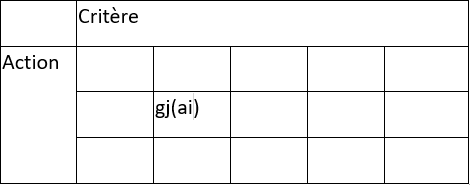
\includegraphics{aide_multicrit_decision/approche_surclassement.png}
\end{center}
\caption{approche de sur-classement}
\end{figure}

Cette approche englobe plusieurs méthodes « ELECTRE, PROMETHEE, ORESTE, MELCHIOR, TACTIC, ...»

Elles sont généralement utilisées quand :

\begin{itemize}
\item un critère au moins n’est pas quantitatif
\item les unités des critères sont très hétérogènes et leur codage en une échelle commune est difficile ou artificielle
\item la compensation entre avantages et désavantages sur différents critères n’est pas justifiable
\item des seuils de préférences ou de veto doivent être pris en compte.
\end{itemize}

Dans le cadre de ce travail, j’ai choisi d’utiliser une méthode de sur-classement car dans un processus d’aide à la décision, lors de la construction du modèle d’évaluation, il est rare d’aboutir uniquement à un seul critère correspondant à un point de vue unique sur lequel  le décideur exprimera ses préférences.\\ 
Il est donc nécessaire de considérer plusieurs points de vue dans la suite de la construction du modèle d’évaluation. Et parmi toutes les méthodes de sur-classement, j’ai choisi ELECTRE III car en plus de ses nombreux avantages que je citerai par la suite, la problématique de mon travail est comme spécifié précédemment une problématique de rangement et la méthode d’aide à la décision de sur-classement la plus appropriée à cette problématique est:l' ELECTRE III.

\subsubsection{La méthode ELECTRE}
La méthode d’analyse multicritère ELECTRE III est fondée sur la construction d’un classement d’alternatives, par le biais d’une approche d’agrégation partielle des performances. Cette méthode est ici appliquée à la gestion des promotions et primes pour les salariés.

\paragraph{Présentation}
ELECTRE signifie élimination et choix traduisant la réalité; c’est une famille de méthodes d'analyse multicritères développée en Europe à la fin des années 1960.\\
ELECTRE est une méthode non compensatoire d'aide à la décision multicritère introduite par Bernard Roy dans le but de Pallier les inconvénients de la somme pondérée.\\
Il existe plusieurs évolutions de cette méthode de surclassement « ELECTRE I, ELECTRE II, ELECTRE III … »\\
La méthode ELECTRE I a été élaborée par Bernard Roy en 1968. Avec l'aide de Patrice Bertier, il a ensuite développé la méthode ELECTRE II (B. Roy, P. Bertier 1971).\\
Les méthodes ELECTRE I et II ont été suivies de beaucoup d'autres parmi lesquelles :
\begin{itemize}
\item ELECTRE III (1978) qui utilise une relation de surclassement valuée et une procédure d'exploitation du graphe valué utilisant des techniques proches de celles de manipulation des nombres flous pour modéliser les pseudo-critères, utilisée généralement dans un besoin de classement.
\item ELECTRE IV (1982) est très simple et suppose que tous les critères (en fait des pseudo-critères) sont de même importance. Elle comporte deux relations de surclassement comme ELECTRE II mais un seul jeu de seuils de veto et la notion de concordance est traduite par une notion de majorité de critères en l'absence de toute pondération.
\item MELCHIOR (JP Leclercq 1984) est une méthode proche de ELECTRE II mais purement ordinale : elle utilise des pseudo-critères et utilise une relation d'ordre au lieu de poids pour refléter l'importance relative des critères. ELECTRE IV apparaît comme un cas particulier de MELCHIOR lorsque la relation d'ordre sur les critères est une équivalence.
Celle qui nous intéresse aujourd’hui et qui est la plus approprié à notre modèle d’aide à la décision :c’est ELECTRE III\\

\end{itemize}


\paragraph{Principe de la méthode Electre III}
La méthode Electre-III est une méthode d’analyse multicritère qui permet de résoudre des problèmes de classement, la méthode s’appuie sur la définition d’une relation de sur-classement S permettant de comparer deux actions a et b distinctes. En considérant un ensemble d’actions A= {a1, a2, a3,…,am}, il s’agit de classer les actions en les comparants par pairs. Chaque action est donc comparée aux autres sur la base des critères considérés. L’évaluation des actions est effectuée par une fonction réelle, pour chaque critère on définit l’ensemble des pseudo-critères G={g1,g2,…,gn} contenant l’évaluation de l’action sur l’ensemble des critères, une fonction a valeur réelle ((gj  : A → R).
La relation de sur-classement est noté (aSb) a surclasse b et elle est valide si les arguments d’un décideur d en faveur de la proposition ”a est au moins aussi bon que b” sont suffisamment forts, les arguments en faveur de aSb sont basés sur:
\begin{itemize}
\item Les évaluations de a (g1(a), g2(a), . . . , gp(a)) et de b (g1(b), g2(b), . . . , gp(b))
\item Une information sur les préférences de d (poids, seuils).
\end{itemize}
Sachant que si aucun argument ne peut être trouvé en faveur de aSb ni de bSa	on a l’incomparabilité.
\begin{itemize}
\item aSb et non bSa ⇒aPb (préférence)	
\item non aSb et bSa ⇒ bPa (préférence)
\item aSb et bSa ⇒ aIb (indifférence)
\item non aSb et non bSa ⇒ aQb (incomparabilité)
\end{itemize}

L’importance des critères dans la prise de décision est évaluée par un ensemble de poids W={W1,W2,…,Wn}. Pour cette méthode, les seuils d’indifférence, de préférence et de veto sont fonction de l’évaluation de l’action pour chaque critère. Pour une action a, évaluée par gj(a) pour le critère j, dans ce cas le seuil d’indifférence est noté qj(gj(a)), le seuil de préférence par pj(gj(a)) de sorte que :
\begin{itemize}
\item aPjb	⇔	|gj (a) − gj (b)| ≥ pj
\item aIjb	⇔	|gj(a) − gj(b)| ≤ qj
\item aQjb	⇔	qj  < gj (a) − gj (b) < pj
\end{itemize}

\begin{figure}[!h]
\begin{center}
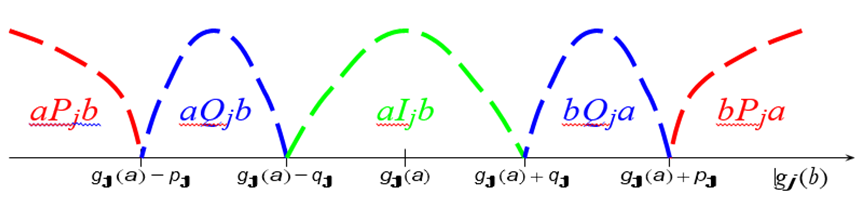
\includegraphics{aide_multicrit_decision/intervales_pref_inconp_indif.png}
\end{center}
\caption{approche de sur-classement}
\end{figure}

Cas particuliers:
\begin{itemize}
\item pj  = qj : quasi-critère,
\item qj  = 0 :	pré-critère,
\item pj  = qj  = 0 : vrai-critère.
\end{itemize}

La méthode Electre III s’appuie sur les étapes  suivantes :

Pour que aSb soit validée, il faut que les deux conditions suivantes soient vérifiées :
\begin{enumerate}
\item Condition  de concordance : une majorité de critères doit être en accord avec aSb (principe majoritaire),
\item Condition de non-discordance : aucun des critères non concordants ne doit réfuter fortement aSb (principe de respect des minorités).
\end{enumerate}
On peut mettre en œuvre ces principes de diverses manières comme on peut  imposer des niveaux d’exigence plus ou moins fort.

\paragraph{Évaluation des indices de concordance :}

la concordance partielle examine la contribution de chaque critère à la proposition aSb, il est obtenu comme suit :\\
Indice de concordance partielle cj (a, b) ∈ [0, 1], (j = 1, . . . , p) tel que :
\begin{itemize}
\item cj (a, b) = 0 ssi gj n’est pas du tout en faveur de aSb
\item cj (a, b) = 1 ssi gj est totalement en faveur de aSb
\item cj (a, b) ∈]0, 1[ ssi gj est partiellement en faveur de aSb
\end{itemize}
	ce qui peut se formuler par :
                      
\[
    c_{j}(a, b)= 
\begin{cases}
    1 ,& \text{if } g_{j}(a) \geq g_{j}(b) - q_{j}\\
    0 ,& \text{if } g_{j}(a) \leq g_{j}(b) - p_{j}\\
    \frac{p_{j} - (g_{j}(b)-g_{j}(a))}{p_{j} - q_{j}}  ,              & \text{sinon}
\end{cases}
\]

\begin{figure}[!h]
\begin{center}
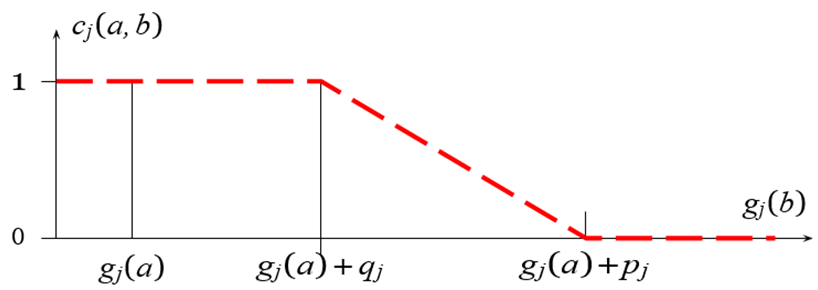
\includegraphics{aide_multicrit_decision/conc_partielle.png}
\end{center}
\caption{Concordance partielle}
\end{figure}

\paragraph{Calcul de l’indice de concordance global :}
la concordance globale apprécie la contribution de l’ensemble des critères à l’affirmation aSb
L’indice de concordance globale C(a, b) ∈ [0, 1]  tel que:
\begin{itemize}
\item C(a, b) = 0 lorsqu’aucun critère n’est en faveur de aSb
\item C(a, b) = 1 lorsque tous les critères sont en faveur de aSb
\item C(a, b) ∈]0, 1[ lorsque “certains” critères sont en faveur de aSb
\end{itemize}

Ce qui peut se formuler par :\\
\[
C(a, b) = \sum_{j=1}^{p}w_{j}c_{j}(a, b)
\]
\[\text{avec } w_{j}  \text{le poids associé au critère  } g_{j},  \sum_{j=1}^{p}w_{j} = 1\]

\paragraph{Évaluation des indices de discordance }


Parmi les critères en désaccord avec aSb, certains peuvent exprimer une forte opposition, un veto qui conduit à invalider aSb, A chaque critère gj , on associe un seuil de veto vj  tel que si gj (a) < gj (b) − vj  pour un j  donné, alors on rejette aSb (quelle que soit l’importance de la coalition concordante),  il est obtenu comme suit :

On définit, sur chaque critère, un indice de discordance partielle dj (a, b) ∈ [0, 1] tel que :
\begin{itemize}
\item dj (a, b) = 0 si gj  ne s’oppose pas à aSb
\item dj (a, b) = 1 si gj  s’oppose totalement à aSb
\item dj (a, b) ∈]0, 1[ si gj  s’oppose en partie à aSb
\end{itemize}

ce qui peut se formuler par :
\[
    d_{j}(a, b)= 
\begin{cases}
    1 ,& \text{if } g_{j}(b) - g_{j}(a) \geq  v_{j}\\
    0 ,& \text{if } g_{j}(b) - g_{j}(a) \leq  p_{j}\\
    1 - \frac{v_{j} - (g_{j}(b)-g_{j}(a))}{v_{j} - p_{j}}  ,              & \text{sinon}
\end{cases}
\]

\begin{figure}[!h]
\begin{center}
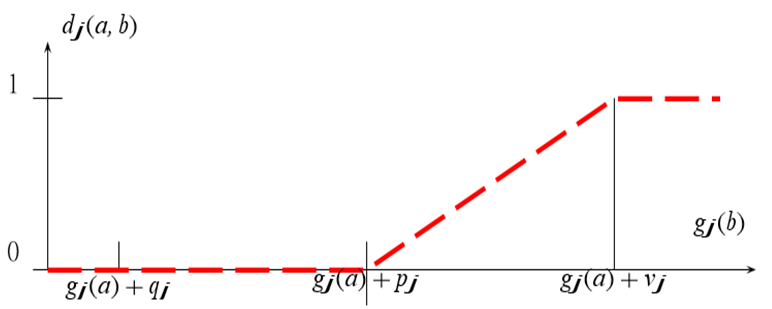
\includegraphics{aide_multicrit_decision/disc_partielle.png}
\end{center}
\caption{Discordance partielle}
\end{figure}

\paragraph{Calcul de l’indice de crédibilité et définition de la relation de sur-classement floue}
Dans Electre III, une relation de sur-classement floue est définie par l’indice de crédibilité $\sigma$(a, b) ∈ [0, 1]
\begin{itemize}
\item si aucun critère n’est discordant $\sigma$(a, b) = C(a, b)
\item si un/plusieurs critère(s) est/sont discordant(s) $\sigma$(a, b) < C(a, b)
\item si dj (a, b) = 1 pour un critère alors $\sigma$(a, b) = 0
\end{itemize}
  
ce qui peut se formuler par :

\[
\sigma(a, b) = C(a, b)\Pi_{j\in\overline{F}}\frac{1-d_{j}(a, b)}{1-C(a,b)} \in [0,1]
\]
\[\text{avec } \overline{F} = \text{\{}{j \in F  \text{ tel que } d_{j}(a, b) > C(a, b)}\text{\}}\]
\newpage
\paragraph{Comparer les indices pour avoir le classement}
On compare à la fin entre les différents indices de crédibilité $\sigma$(a, b) de chaque action et on  garde le plus grand à chaque fois c’est-à-dire on sélectionne la meilleure action et on classe les  actions de la meilleure à la moins bonne, on parle ici de distillation descendante.

\paragraph{Avantages et inconvénients}
\begin{itemize}
\item Tout d’abord, cette approche d’analyse multicritère est fondée sur une démarche constructive. En effet, le contexte dans lequel les outils multicritères sont utilisés est voué à évoluer au cours du temps et de l’information acquise.
\item Ensuite, cette méthode permet de prendre en compte les poids donnés aux critères de jugement. Cette étape de pondération permet aux différents acteurs de donner leurs opinions et d’exprimer d’éventuelles différences de jugement.
\item La simplicité de la méthode vu qu’elles reposent sur des concepts naturels, tels « d'accord » ou « pas d'accord ».
\item Enfin, ELECTRE III est une méthode multicritère fondée sur les principes de la logique floue, permettant de prendre en compte les incertitudes liées aux calculs et à l’évaluation des performances à travers l’utilisation de pseudo-critères. C’est l’une des principales caractéristiques de la méthode de pouvoir traiter, du fait de l’existence des seuils, d’évaluations dont la définition est difficile.
\item L’inconvénient avec ELECTRE est sa grande complexité et son recourt important aux valeurs numériques qui la rapprochent des méthodes d'utilité.
\end{itemize}



\section{Conclusion}
Ce chapitre présente la notion d’aide à la décision, et plus particulièrement l’aide à la décision multicritère et les deux méthodes que j’ai implémenté dans le cadre de ce travail, dans la section suivante, nous allons voir la partie conception et implémentation de l’outil d’aide à la décision pour le classement des salariés.








